\documentclass[12pt]{article}
\usepackage[utf8]{inputenc}
\usepackage{acronym}
\usepackage{amsmath}
\usepackage{amsfonts}
\usepackage{amssymb}
\usepackage{booktabs}
\usepackage{braket}
\usepackage{changepage}
\usepackage{enumitem}
\usepackage{fancyhdr}
\usepackage{graphicx}
\usepackage{geometry}
\usepackage[none]{hyphenat}
\usepackage{lipsum}
\usepackage{multicol}
\usepackage[numbers]{natbib}
\usepackage{parskip}
\usepackage{subcaption}
\usepackage{tabularx}
\usepackage{tcolorbox}
\geometry{a4paper, margin=1in}
\setlength{\columnsep}{0.7cm}
\newcommand{\vctr}[1]{\ensuremath{\mathbf{#1}}}
\newcommand{\vctrg}[1]{\mbox{\boldmath{$#1$}}}
\newcommand{\unitr}[1]{\ensuremath{\mathbf{\hat{#1}}}}
\newcommand{\depar}[2]{\ensuremath{\frac{\partial#1}{\partial#2}}}
\newcommand{\depars}[2]{\ensuremath{\frac{\partial^{2}#1}{\partial#2^{2}}}}
\newcommand{\perme}{\ensuremath{\epsilon_{0}}}
\newcommand{\permm}{\ensuremath{\mu_{0}}}
\newcommand{\unitrg}[1]{\mbox{\boldmath{$\hat{#1}$}}}
%\numberwithin{equation}{section} % This line resets equation numbering when starting a new section.


\title{EP716: Reactor Thermal-Hydraulics Design}
\author{Md. Ariful Islam \\ Email: islamm65@mcmaster.ca \\ Department of Engineering Physics, McMaster University}
\date{}

\begin{document}

\maketitle

\rule{\textwidth}{0.4pt}

\section*{Problem 1}

Show that if water passes through the core of a BWR reactor at the rate of $w$ kg/s then the 
mass flow of steam produced will be given by the following relation: 
\begin{equation*}\label{eq:1}
w_{e}={\frac{q-w(h_{f}-h_{i n})}{h_{f g}}}
\end{equation*}

where, $q$ is the thermal power of the reactor; $h_f$ and $h_{in}$ are respectively enthalpy of saturated water leaving the core and enthalpy of water entering the core; and $h_{fg}$ is latent heat of vapourization.

\section*{Answer}

In a BWR, the water entering the core absorbs heat, and a portion of it turns into steam. The energy balance can be written as:
\begin{equation}\label{eq:2}
    q = Energy\ to\ heat\ water + Energy\ to\ produce\ steam
\end{equation}

\begin{enumerate}
    \item Energy to heat water from $h_{in}$ to $h_f$:
    \begin{equation}\label{eq:3}
        E_{heating} = w(h_f - h_{in})
    \end{equation}
    \item Energy to produce steam (latent heat of vaporization):
    \begin{equation}
        E_{vaporization} = w_e \cdot h_{fg}
    \end{equation}
\end{enumerate}

The total thermal power $q$ is the sum of these two components:
\begin{equation}
    q = w(h_f - h_{in}) + w_e \cdot h_{fg}
\end{equation}

Rearrange the equation to solve for $w_e$:
\begin{tcolorbox}
    \begin{equation}
\begin{gathered}
    w_e \cdot h_{fg} = q - w(h_f - h_{in}) \\
    w_{e}={\frac{q-w(h_{f}-h_{i n})}{h_{f g}}}
\end{gathered}
\end{equation}
\end{tcolorbox}
%%--------------------------------------------------------------

\section*{Problem 2}

The heat flux in a reactor core has the following shape: decreases linearly and symmetrically  from the core centre to both ends of the core, from 630 $kW/m^2$ to 315 $kW/m^2$. The fuel rods  have diameter of 1.3 cm, and are 1.8 m long. Water enters the core at a temperature of 65$^{\circ}c$ and flows through the core at a rate of 0.05 $kg/s$ per rod. The heat transfer coefficient is 5.6 $KW / m^2.^{\circ}c$. Calculate the temperatures of the coolant, fuel rod surface, and fuel rod centre at  the entrance of the channel, at the center of the channel, and at the channel exit.

\section*{Answer}

Given data:
\begin{itemize}
    \item Maximum surface heat flux (at center): $q^{\prime \prime}_{max} = 630 \frac{KW}{m^2}$
    \item Fuel rod diameter: $D = 0.013 \: m$
    \item Flow area, $A_f = \frac{\pi \cdot D^2}{4} = 0.0001327 \; m^2$
    \item Fuel rod length: $L = 1.8 \; m$
    \item Mass flow rate: $w = 0.05 \; kg/s$
    \item Inlet temperature: $T_{in} = 65^{\circ} c$
    \item Surface heat transfer coefficient $h_S = 5.6 \; \frac{KW}{m^2 \cdot ^{\circ} c} = 5600 \frac{W}{m^2 \cdot ^{\circ} K}$
    \item Water specific heat: $c_p = 4180 \; J/kg \cdot ^{\circ} c$
\end{itemize}

\textbf{Coolant temperature at the center of the channel, and at the channel exit}:

\begin{enumerate}
    \item The coolant temperature in the middle of the fuel element for $z=0$ has the following form \cite{popov2017th}:
    \begin{equation}
    \begin{gathered}
        T_{c, mid}=T_{c,i n}+\frac{\left(q^{\mathrm{\prime \prime }}\right)_{\mathrm{max~}}A_{f}L}{\pi\,w c_{p}} \\
        T_{c, mid} = \boxed{65.23 ^{\circ} c}
    \end{gathered}
    \end{equation}
    \item The exit temperature of the coolant can be obtained using the following equation \cite{popov2017th}:
    \begin{equation}
        \begin{gathered}
            T_{c,o u t}=T_{c,i n}+{\frac{2\left(q^{\prime \prime }\right)_{\mathrm{max}}A_{f}L}{\pi\,w C_{p}}} \\
            T_{c,o u t}= \boxed{65.46 ^{\circ} c}
        \end{gathered}
    \end{equation}
Axial temperature distribution for coolant along the channel height $[-L/2, \;L/2]$ as follows :

\begin{figure}[h!]
\centering
    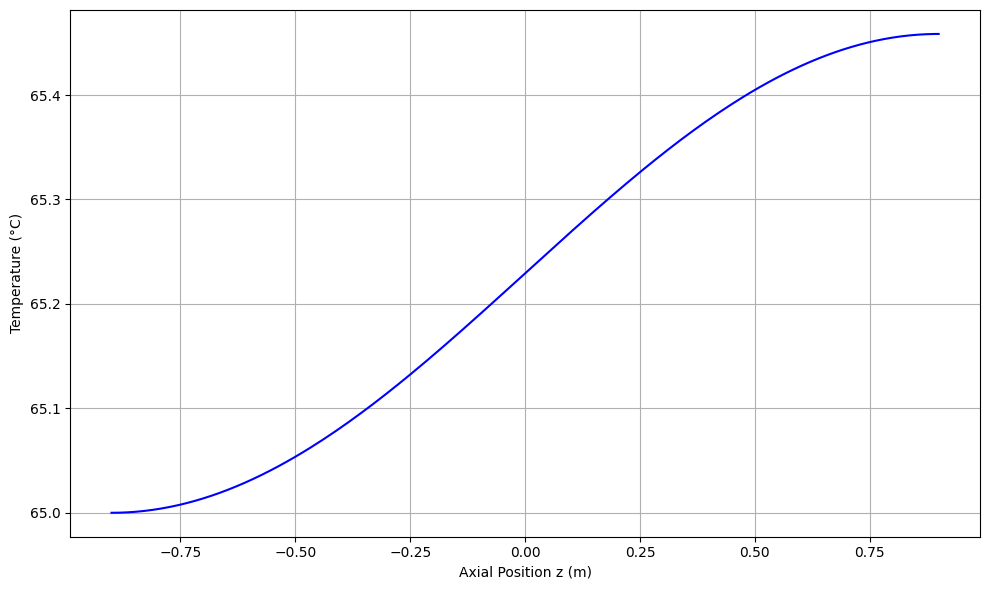
\includegraphics[width=0.8\textwidth]{axial_temperature_distribution.png}
    \caption{Coolant Temperature $T_c(z)$}
    \label{1}
\end{figure}
    
\end{enumerate}

\textbf{Fuel Surface and Centerline temperature at the channel entrance, center of the channel, and at the channel exit}:

Fuel surface temperature along the channel length can be calculated using the following formula,
\begin{equation}\label{8}
    \begin{gathered}
        T_{f,S}=T_{c}+R_{f,S}L\biggl[\biggl({q}^{\prime \prime}\biggr)_{\mathrm{max}}\,{A}_{f}\,\mathrm{cos}\biggl(\frac{\pi*z}{L}\biggr)\biggr] , \; where \\
        T_c = T_{c,i n}+\frac{\left(q^{\prime \prime}\right)_{\mathrm{max}}V_{f}}{\pi\,w c_{p}}\left[1+\mathrm{sin}\left(\frac{\pi*z}{L}\,\right)\right], \; and \\
        R_{f,S}=\left(\frac{1}{h_{G}r_{F}}+\frac{t_{G}+t_{C}}{k_{C}\left(r_{F}+t_{G}\right)}+\frac{1}{h_{S}\left(r_{F}+t_{G}+t_{S H}\right)}\right)
    \end{gathered}
\end{equation}

Since no gap, cladding, sheath data are given $t_G = t_C = t_{SH} = 0$, 
\begin{equation*}
    R_{f,S}={\frac{1}{h_{S}(r_{F}+t_{G}+t_{S H})}}
\end{equation*}

Solving Eqn \ref{8}, fuel surface temperature at entrance, mid, and exit positions are;
\begin{tcolorbox}
\begin{equation*}
    \begin{gathered}
        T_{{f, S}_{(z=-L/2)}} = 65 ^{\circ}c \\
        T_{{f, S}_{(z=0)}} = 69.3644 ^{\circ}c \\
        T_{{f, S}_{(z=L/2)}} = 65.458 ^{\circ}c
    \end{gathered}
\end{equation*}

\end{tcolorbox}
For fuel centerline temperature distribution, we can use following equation;
\begin{equation}\label{9}
    \begin{gathered}
        T_{f,C L}=T_{c,i n}+\frac{\left(q^{\prime \prime}\right)_{\mathrm{max}}A_{f}L}{\pi\,w C_{p}}\Bigg[1+\mathrm{sin}\Bigg(\frac{\pi\,z}{L}\Bigg)\Bigg]+\left(q^{\prime \prime}\right)_{\mathrm{max}}A_{f}L R_{f,C L}\cos\Bigg(\frac{\pi\,z}{L}\Bigg) , \; where \\
        R_{f,C L}=\left(\frac{1}{2\overline{{{k}}}_{f}}+\frac{1}{h_{G}r_{F}}+\frac{t_{G}+t_{C}}{k_{C}\left(r_{F}+t_{G}\right)}+\frac{1}{h_{S}\left(r_{F}+t_{G}+t_{S H}\right)}\right)
    \end{gathered}
\end{equation}

Solving Eqn \ref{9}, fuel centerline temperature at entrance, mid, and exit positions are;
\begin{tcolorbox}
\begin{equation*}
    \begin{gathered}
        T_{{f, CL}_{(z=-L/2)}} = 65 ^{\circ}c \\
        T_{{f, CL}_{(z=0)}} = 94.45 ^{\circ}c \\
        T_{{f, CL}_{(z=L/2)}} = 65.458 ^{\circ}c   
    \end{gathered}
\end{equation*}
\end{tcolorbox}
% \begin{equation*}
%     \begin{gathered}
%         T_{{f, CL}_{(z=-L/2)}} = 65 ^{\circ}c \\
%         T_{{f, CL}_{(z=0)}} = 94.45 ^{\circ}c \\
%         T_{{f, CL}_{(z=L/2)}} = 65.458 ^{\circ}c   
%     \end{gathered}
% \end{equation*}

Using Eqn. \ref{8} and \ref{9}, fuel surface and centerline temperature distribution along the channel height $[-L/2, \;L/2]$ is,

\begin{figure}[h!]
\centering
    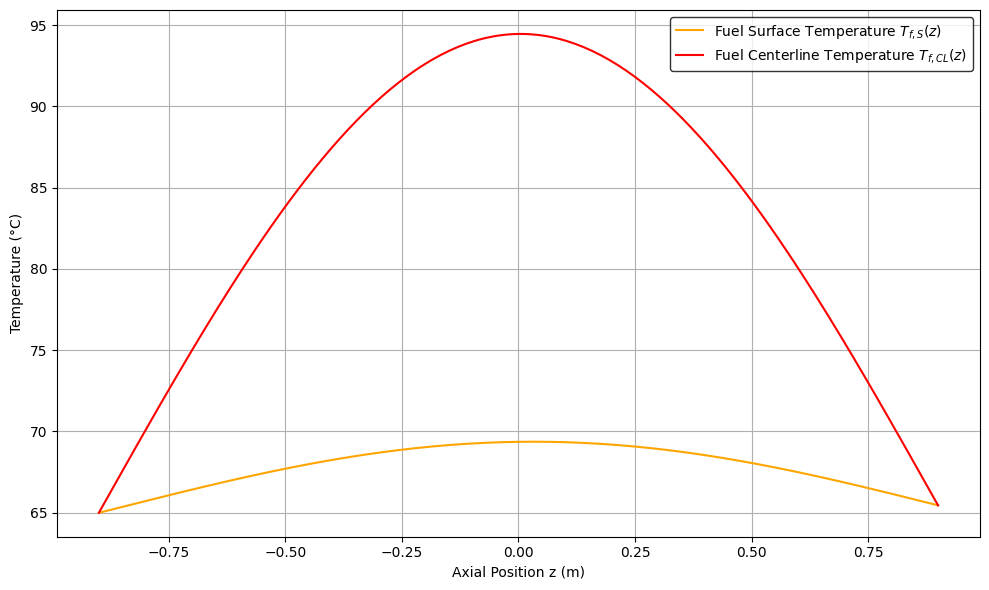
\includegraphics[width=0.8\textwidth]{surface_temperature_distribution.png}
    \caption{Fuel Temperature Distribution}
    \label{1}
\end{figure}
%%--------------------------------------------------------------

\section*{Problem 3}
For a PWR reactor with flow is evenly distributed across the core, the following parameters are given: pressure 15.5 MPa; inlet temperature 286 $^\circ c$  exit temperature 324 $^\circ c$; linear power rate 
at midplane (averaged radially across the core) is 17.8 $kW/m$;  number of fuel pins 50,952; core flow rate 17.4 $Mg/s$; fuel outside diameter 9.5 mm; clad thickness 0.57 mm; gap 0.08 mm; pitch 12.5 mm; fuel rod height 4 m; active fuel height 3.66 m. Calculate how much power can be extracted from this PWR if: (a) the coolant exit temperature is to remain subcooled. (b) the  maximum clad temperature is to remain below saturation temperature, and (c) the fuel  maximum temperature is to remain below 2400 $^\circ c$

\section*{Answer}
Given parameters:
\begin{itemize}
    \item Inlet Temp: $T_{in} = 286^{\circ} c$
    \item Exit Temp:  $T_{out} = 324^{\circ} c$
    \item Mass flow rate: $\dot{m} = 17.4 \; Mg/s = 17.4 \times 10^3 \; kg/s$
    \item Specific heat of water (approx.): $c_p = 5.2 \; KJ/kg.K$
    \item Pressure $P=15.5$ MPa
    \item Linear Power Rate at midplane: $17.8 \; KW/m$
    \item Number of fuel pins $N_{\mathrm{pins}}$: 50,952
    \item Fuel rod height = 4 m
    \item Active fuel height $L_{\mathrm{active}}$ = 3.66 m
\end{itemize}

\begin{enumerate}
    \item The total power that can be extracted from this PWR core while keeping the coolant subcooled at the exit is;
\begin{equation}
    \begin{gathered}
        \dot{Q} = \dot{m} \cdot c_p \cdot (T_{out} - T_{in}) \\
        \dot{Q} = 17.4 \times 10^3 \cdot 5.2 \cdot 38 \; KW
        \dot{Q} = \boxed{3438.24 \;MW_{th}}
    \end{gathered}
\end{equation}

\item \begin{itemize}
    \item Coolant pressure = 15.5 MPa, Saturation temperature $\approx 345 ^{\circ} c$
    \item Allowable maximum clad surface temperature $T_{clad, max} = 345 ^{\circ} c$
\end{itemize}

So, \[\Delta T_{\mathrm{clad,coolant}}=T_{\mathrm{clad, max}}-T_{c,\mathrm{out}}=345-324=21^{\circ}C\]. Using surface convective heat transfer coefficient $h_S$ from \cite{popov2017th} \[h_S = 4.5\ W/{\mathrm{cm}}^{2}\cdot\mathrm{K}=45.000\ \mathrm{W/m}^{2}\cdot\mathrm{K}\], we can now calculate $q^{\prime \prime}_{max}$; \[q_{\mathrm{max}}^{\prime\prime}=h_S\cdot\Delta T=45,000\cdot(345-324)=45,000\cdot21 = 945000 \; W/m^2\]. Using outer fuel rod diameter $d_{fuel} = 9.5 \; mm = 0.0095 \; m$ we can now calculate linear power; \[P_{\mathrm{linear}}=q_{\mathrm{max}}^{\prime \prime}\cdot\pi d_{\mathrm{fuel}}=945,000\cdot\pi\cdot0.0095\approx 28.20 \times 10^3 \; W/m\] The maximum power output while keeping cladding temperature below saturation temperature is,
\begin{equation}
    \begin{gathered}
        P_{\mathrm{total}}=P_{\mathrm{linear}}\cdot L_{\mathrm{active}}\cdot N_{\mathrm{pins}} = \boxed{5259.54 \; MW_{th}}
    \end{gathered}
\end{equation}

\item Using fuel centerline temperature equation, 
\begin{equation*}
    T_{f,C L}=T_{c,i n}+\frac{\left(q^{\prime \prime}\right)_{\mathrm{max}}A_{f}L}{\pi\,w C_{p}}\Bigg[1+\mathrm{sin}\Bigg(\frac{\pi\,z}{L}\Bigg)\Bigg]+\left(q^{\prime \prime}\right)_{\mathrm{max}}A_{f}L R_{f,C L}\cos\Bigg(\frac{\pi\,z}{L}\Bigg)
\end{equation*}

At the midplane , where $z=0$, trigonometric terms simplify to $sin (0)=0, \; cos(0) = 1$. So the formula becomes:
\begin{equation*}
    \begin{gathered}
        T_{f,{\mathrm{C L}}}=T_{\mathrm{cin}}+{\frac{q_{\mathrm{max}}^{\prime\prime}\cdot A_{f}\cdot L}{\pi w c_{p}}}+q_{\mathrm{max}}^{\prime\prime}\cdot A_{f}\cdot L\cdot R_{f,C L} \\
        T_{f,\mathrm{C L}}=T_{c,\mathrm{in}}+q_{\mathrm{max}}^{\prime\prime}\cdot A_{f}\cdot L\cdot\left({\frac{1}{\pi w c_{p}}}+R_{f,C L}\right) \\
        q_{\mathrm{max}}^{\prime\prime}={\frac{T_{f,\mathrm{C L}}-T_{c, i n}}{A_{f}\cdot L\cdot\left({\frac{1}{\pi w c_{p}}}+R_{f,C L}\right)}}
    \end{gathered}
\end{equation*}

Using known values,
\begin{itemize}
    \item $T_{c , \; in} = 286 ^{\circ} c$
    \item $T_{f, \; CL} = 2400 ^{\circ} c$, as fuel maximum temperature is to remain below $2400 ^{\circ} c$
    \item Flow area $A_f = 0.1092 \; m^2$
    \item Gap thickness $t_{gap} = 0.08e-3 \; m$
    \item Fuel radius $r_f = 0.00475 \; m$
\end{itemize}

\begin{equation}
    \begin{gathered}
        q_{\mathrm{max}}^{\prime\prime}= 1.149 \times 10^6 \; W/m^2 \\
        P_{\mathrm{linear}}=q_{\mathrm{max}}^{\prime \prime}\cdot\pi d_{\mathrm{fuel}} = 34.31 \times 10^3 \; W/m^2 \\
        P_{\mathrm{total}}=P_{\mathrm{linear}}\cdot L_{\mathrm{active}}\cdot N_{\mathrm{pins}} = \boxed{6398.47 \; MW_{th}}
    \end{gathered}
\end{equation}
\end{enumerate}

%%--------------------------------------------------------------

\section*{Problem 4}

Water at 14 MPa and 322 $^\circ c$ leaves a PWR reactor vessel via a 0.74-m ID outlet primary  coolant pipe with an average flow velocity of 15 m/s. Calculate (a) mass flow rate out of this  pipe; (b) Reynolds number; (c) assuming the water returns to the reactor vessel at the same  pressure and velocity but at temperature of 290 $^\circ c$, calculate the ID of the inlet primary pipe

\section*{Answer}
Given data:
\begin{itemize}
    \item Outlet pipe diameter: $D_{out} = 0.74 \; m$
    \item Average flow velocity: $v=15 \; m/s$
    \item Pressure $P=14 \; MPa$
    \item Outlet temperature: $T_{out} = 322 ^{\circ} c$
    \item Inlet temperature: $T_{in} = 290 ^{\circ} c$
\end{itemize}

\begin{enumerate}
    \item The mass flow rate is given by: \[{\dot{m}}=\rho\cdot A\cdot v\] where 
    \begin{itemize}
        \item $A = \frac{\pi}{4} \cdot D^2$ is the cross-sectional area
        \item $\rho$ is the density of water at 14 MPa and 322 $^{\circ} c \approx 670.23 \; kg/m^3$ [From NIST ] 
    \end{itemize}

So mass flow rate out of this pipe,
\begin{equation}
    \begin{gathered}
        A={\frac{\pi}{4}}(0.74)^{2}\approx 0.43\,{\mathrm{m}}^{2} \\
        \dot{m}=670.23\cdot0.43\cdot 15 \approx \boxed{4322.98 \; kg/s}
    \end{gathered}
\end{equation}
\item Reynolds number; \[Re = \frac{\rho \cdot v \cdot D}{\mu}\] Dynamic viscosity at 14 MPa and 322 $^{\circ} c$, from NIST: \[\mu \approx 7.8850 \times 10^{-5} \; Pa.s\] 
\begin{equation}
    Re = \frac{670.23 \cdot 15 \cdot 0.74}{7.8850 \times 10^{-5}} = \boxed{9.44 \times 10^7}
\end{equation}

This is a very high Reynolds number, indicating fully turbulent flow.
\item Since mass flow rate $\dot{m}$ is conserved; 
\begin{equation*}
    {\dot{m}}=\rho_{i n}\cdot A_{i n}\cdot v\Rightarrow A_{i n}={\frac{\dot{m}}{\rho_{i n}\cdot v}}
\end{equation*}

At 14 MPa, 290$^{\circ}$c, $\rho_{in} \approx 743.56 \; kg/m^3$. Then 
\begin{equation}
    \begin{gathered}
        A_{i n}={\frac{4322.98}{743.56 \cdot 15}} = 0.3876\,\mathrm{m^{2}} \\
        D_{i n}={\sqrt{\frac{4A}{\pi}}}={\sqrt{\frac{4\times 0.3876}{\pi}}} = \boxed{0.7025 \, m}
    \end{gathered}
\end{equation}
\end{enumerate}

%-----------------
% Bibliography
%-----------------

\bibliographystyle{IEEEtran} % You can choose a different style if needed
\bibliography{ref} % This refers to the Bibliography.bib file

\end{document}
